\documentclass[a4paper]{book} %{article}

\usepackage{fullpage} % Package to use full page
\usepackage{parskip} % Package to tweak paragraph skipping
\usepackage{tikz} % Package for drawing
\usepackage{amsmath}
\usepackage{hyperref}
\usepackage[numbered]{bookmark} % For numbering of challenges in bookmark pane of PDF viewer
\def\UrlBreaks{\do\/\do-}
\usepackage[absolute]{textpos}
\setlength{\TPHorizModule}{1mm}
\setlength{\TPVertModule}{1mm}
\usepackage{tikz}
\usepackage{siunitx}
\usepackage{bm} % Bold math \bm command
\usepackage{datetime} % Time
\usepackage[UKenglish]{isodate} % UK-format date
\usepackage{ctable} % Thick table lines
\usepackage{amssymb} % Realspace symbol


\newcommand{\six}[1]{\SI[parse-numbers=false]{X}{#1}}
\graphicspath{{Images/}}

% Discussion times
\newcommand{\disctime}{10:30 to 12:00 }
\newcommand{\discdays}{Wednesdays }
\newcommand{\discroom}{W4-529}
\newcommand{\discexam}{8th February 2017} % Final exam
\newcommand{\course}{Fourier Analysis }
\newcommand{\courseurl}{fourier-analysis}
\newcommand{\nensei}{3rd}
\newcommand{\timebox}{\vfill Study-time (from end of previous challenge to end of this challenge): \underline{\hspace{1cm} minutes}}
\newcommand{\assstart}{26 October}


\newcommand{\hash}[2]{MD5(#1\_X) = #2\ldots}
% Add timetable?

\title{Fourier Analysis\\Autumn 2016}
\author{James Cannon, Kyushu University}
\date{\today}

\begin{document}

\begin{titlepage}
    \begin{center}
        \vspace*{1cm}

        \Huge
        \textbf{Fourier Analysis}

        Autumn 2016

        \vspace{1.5cm}
        \Large
        Last updated:\\\today \ at \currenttime

        \vspace{4.0cm}
        \LARGE
        James Cannon\\Kyushu University
         \vfill

        \normalsize
        \url{http://www.jamescannon.net/teaching/\courseurl}
        \vspace{0.2cm}
        \small
        \url{http://raw.githubusercontent.com/NanoScaleDesign/FourierAnalysis/master/fourier_analysis.pdf}
        \vspace{0.5cm}

        License: \emph{CC BY-NC 4.0}.

    \end{center}
\end{titlepage}

\setcounter{chapter}{-1}

\tableofcontents

\chapter{Course information}
\newpage
\section{This course}
This is the Autumn 2016 \course course studied by \nensei-year undegraduate international students at Kyushu University.

\subsection{How this works}
\begin{itemize}
    \item In contrast to the traditional lecture-homework model, in this course the learning is self-directed and active via publicly-available resources.
    \item Learning is guided through solving a series of carefully-developed challenges contained in this book, coupled with suggested resources that can be used to solve the challenges with instant feedback about the correctness of your answer.
    \item There are no lectures. Instead, there is discussion time. Here, you are encouraged to discuss any issues with your peers, teacher and any teaching assistants. Furthermore, you are encouraged to help your peers who are having trouble understanding something that you have understood; by doing so you actually increase your own understanding too.
    \item Discussion-time is from \disctime on \discdays at room \discroom.
    \item Peer discussion is encouraged, however, if you have help to solve a challenge, always make sure you do understand the details yourself. You will need to be able to do this in an exam environment. If you need additional challenges to solidify your understanding, then ask the teacher. The questions on the exam will be similar in nature to the challenges. If you can do all of the challenges, you can get 100\% on the exam.
    \item Every challenge in the book typically contains a \textbf{Challenge} with suggested \textbf{Resources} which you are recommended to utilise in order to solve the challenge. A \textbf{Solution} is made available in encrypted form. If your encrypted solution matches the encrypted solution given, then you know you have the correct answer and can move on. For more information about encryption, see section \ref{sec:hashes}. Occasionally the teacher will provide extra \textbf{Comments} to help guide your thinking.
    \item For deep understanding, it is recommended to study the suggested resources beyond the minimum required to complete the challenge.
    \item The challenge document has many pages and is continuously being developed. Therefore it is advised to view the document on an electronic device rather than print it. The date on the front page denotes the version of the document. You will be notified by email when the document is updated.
    \item A target challenge will be set each week. This will set the pace of the course and defines the examinable material. It's ok if you can't quite reach the target challenge for a given week, but then you will be expected to make it up the next week.
    \item You may work ahead, even beyond the target challenge, if you so wish. This can build greater flexibility into your personal schedule, especially as you become busier towards the end of the semester.
    \item Your contributions to the course are strongly welcomed. If you come across resources that you found useful that were not listed by the teacher or points of friction that made solving a challenge difficult (there's no such thing as ``you should have learned it in high-school'' - you're probably not the only one with that specific problem), please let the teacher know about it!
\end{itemize}

\subsection{Assessment}
In order to prove to outside parties that you have learned something from the course, we must perform summative assessments. This will be in the form of

\begin{equation*}
    \text{overall score} = (0.5 E_F + 0.3 E_M + 0.2 C) (0.9 + P/10)
\end{equation*}

Your final score is calculated as Max($E_F$, overall score), however you must pass the final exam ($\ge 60\%$) to pass the course.

\begin{itemize}
    \item $E_F$ = \% correct on final exam
    \item $E_M$ = \% correct on mid-term exam
    \item $C$ = \% grade on course-work
    \item $P$ = participation calculated as $P = (F/N_D)(A/N_D)(L/N_L)$ where each terms is as follows
        \begin{itemize}
            \item $F$ = Number of weeks where feedback form is submitted 24 hours before discussion time (including spreadsheet update).
            \item $A$ = Number of discussion classes attended
            \item $N_D$ = Number of discussion classes held
            \item $L$ = Number of times that your collected challenge log is satisfactory. This means:
                \begin{itemize}
                    \item Available on request.
                    \item Your calculations are clearly shown.
                    \item It corresponds to your spreadsheet.
                    \item It contains evidence of trying to keep up with the target challenge. Short-term fluctuations in completing challenges are fine (eg, if you had trouble understanding material to overcome some challenges this week) but the long-term trend should be more-or-less to keep up with the target challenge.
                \end{itemize}
            \item $N_L$ = Number of times that your challenge log is collected.
        \end{itemize}
\end{itemize}

Note that $P$ is only calculated from \assstart. If $N - F \le 2$ then $F$ is treated as being equal to $N$ (ie, you can forget twice). You can be counted as attending the class even if you are not present if the reason for not attending is unavoidable (eg, health reasons) and you inform the teacher in advance.

Please also note that, since late arrivals disrupt the class by preventing intended pairing of students, attendance of a discussion class will be only counted as partial if you are more than a minute or two late (eg, 9 minutes late out of a 90-minute discussion class will count as attending only 90\% of the class). Therefore, if you will be unavoidably late, you need to let the teacher know in advance. To allow for unexpected delays, for up to two late arrivals you will be considered to have attended 100\% of the discussion time.



\subsection{What you need to do}
\begin{itemize}
    \item Prepare a challenge-log in the form of a workbook or folder where you can clearly write the calculations you perform to solve each challenge. This will be a log of your progress during the course and will be occasionally reviewed by the teacher.
    \item You will need to maintain a google spreadsheet detailing your work and progress. The purpose of this spreadsheet is to help the teacher optimise the discussion-time. Please ensure that it is up-to-date 24 hours before each discussion-time starts. It is fine for you to continue to work on challenges and update the spreadsheet after the 24-hour deadline.
    \item You also need to submit a brief report at \url{https://goo.gl/forms/Djl4FEZcJLMpipsY2} 24 hours before the discussion time starts. Here you can let the teacher know about any difficulties you are having and if you would like to discuss anything in particular.
    \item Please bring a wifi-capable internet device to class, as well as headphones if you need to access online components of the course during class. If you let me know in advance, I can lend computers and provide power extension cables for those who require them (limited number).
\end{itemize}

\subsection{Details about the spreadsheet}
To get started:
\begin{enumerate}
    \item Log into google
    \item Open \url{http://bit.ly/2cPYyQY}
    \item File $\rightarrow$ Make a copy [$\rightarrow$ rename] $\rightarrow$ ok
    \item Click ``Share'' (top right)
    \item Click ``Get shareable link''
    \item Set ``Anyone with the link can edit''
    \item Copy sharing address
    \item Send an email to cannon@mech.kyushu-u.ac.jp containing
    \begin{enumerate}
       \item Subject: \course registration
       \item Your name
       \item Student number
       \item The link to your copy of the google sheet
    \end{enumerate}
\end{enumerate}

Using the spreadsheet:

\begin{itemize}
    \item Enter the appropriate challenge number. For example, for challenge 1.4, enter ``1'' in the \textbf{Section} column and ``4'' in the \textbf{Challenge} column.
    \item After successfully completing a challenge, please enter any particular friction points that you experienced (if any) so the course can be developed to reduce such friction in the future, as well as any extra resources you recommend (if any).
    \item Please also roughly estimate the amount of effort in required to complete the challenge (starting from when you completed the previous challenge, including any reading, watching videos, looking for resources, writing the answer to the challenge, discussing with peers, etc). This is not used for assessment in any way, but is very valuable in helping the teacher develop the course. Note: Although the column says \textbf{Hours}, please specify the time in terms of \textbf{minutes}.
\end{itemize}

Note: Please do not alter column names, ordering, etc. Just add section and challenge numbering and fill in the columns as appropriate. This is because spreadsheet data is downloaded and automatically analysed, and it breaks if anything is inconsistent.

\newpage
\section{Timetable}

\begin{center}
    \begin{tabular}{|c|c|c|c|}
        \hline
        & \textbf{Discussion} & \textbf{Target} & \textbf{Note} \\ \specialrule{.1em}{.05em}{.05em}
        \textbf{1}  &  3 Oct & -            &                             \\ \hline
        \textbf{2}  & 17 Oct & 2.11         &                             \\ \hline
        \textbf{3}  & 24 Oct & 3.10         &                             \\ \hline
        \textbf{4}  & 31 Oct &              &                             \\ \specialrule{.1em}{.05em}{.05em}
        \textbf{5}  &  7 Nov &              &                             \\ \hline
        \textbf{6}  & 14 Nov &              &                             \\ \hline
        \textbf{7}  & 21 Nov &              &                             \\ \hline
        \textbf{8}  & 28 Nov &              &                             \\ \specialrule{.1em}{.05em}{.05em}
        \textbf{9}  & 5 Dec  &              &                             \\ \hline
        \textbf{10} & 12 Dec &              &                             \\ \hline % NT: Give students more of a rest after the mid-term
        \textbf{11} & 19 Dec &              &                             \\ \specialrule{.1em}{.05em}{.05em}
        \textbf{12} &  9 Jan &              &                             \\ \hline
        \textbf{13} & 16 Jan &              &                             \\ \hline
        \textbf{14} & 23 Jan &              &                             \\ \specialrule{.1em}{.05em}{.05em}
        \textbf{15} & 6 Feb  & Final exam   & Tentative                   \\ \hline
    \end{tabular}
\end{center}

\newpage
\section{Hash-generation}
\label{sec:hashes}

Most solutions to challenges are encrypted using MD5 hashes. In order to check your solution, you need to generate its MD5 hash and compare it to that provided.  MD5 hashes can be generated at the following sites:

\begin{itemize}
    \item Wolfram alpha: (For example: md5 hash of ``q\_1.00'') \url{http://www.wolframalpha.com/input/?i=md5+hash+of+\%22q_1.00\%22}
    \item \url{www.md5hashgenerator.com}
\end{itemize}

Since MD5 hashes are very sensitive to even single-digit variation, you must enter the solution exactly. This means maintaining a sufficient level of accuracy when developing your solution, and then entering the solution according to the format below:

Unless specified otherwise, any number from $0.00$ to $\pm 9999.99$ should be represented as a normal number to two decimal places. All other numbers should be in scientific form. See the table below for examples.

\begin{center}
\begin{tabular}{|l|l|}
    \hline
    \textbf{Solution} & \textbf{Input} \\ \hline
    1 & 1.00 \\
    -3 & -3.00 \\
    -3.5697 & -3.57 \\
    0.05 & 0.05 \\
    0.005 & 5.00e-3 \\
    50 & 50.00 \\
    500 & 500.00 \\
    5000 & 5000.00 \\
    50,000 & 5.00e4 \\
    $5 \times 10^{-476}$ & 5.00e-476 \\
    $5.0009 \times 10^{-476}$ & 5.00e-476 \\
    $-\infty$ & -infinity (never ``infinite'')\\
    $2 \pi$ & $6.28$ \\
    i & im(1.00) \\
    2i & im(2.00) \\
    1 + 2i & re(1.00)im(2.00) \\
    -0.0002548 i & im(-2.55e-4) \\
    1/i = i/-1 = -i & im(-1.00) \\
    $e^{i2\pi}$ [$= cos(2 \pi) + isin(2 \pi) = 1 + i0 = 1$] & 1.00 \\
    $e^{i\pi/3}$ [$= cos(\pi/3) + isin(\pi/3) = 0.5 + i 0.87$] & re(0.50)im(0.87) \\
    Choices in order A, B, C, D & abcd \\
    \hline
\end{tabular}
\end{center}

Entry format is given with the problem. So ``q\_X'' means to enter ``q\_X'' replacing ``X'' with your solution. The first 6 digits of the MD5 sum should match the given solution (MD5(q\_X)= \ldots).

Note that although some answers can usually only be integers (eg, number of elephants), for consistency, to generate the correct hash, the accuracy in terms of decimal places noted above is required.


\chapter{Periods and frequencies}
\section{Period at 50 THz}

\subsection*{Resources}
\begin{itemize}
    \item Video: \url{https://www.youtube.com/watch?v=v3CvAW8BDHI}
\end{itemize}

\subsection*{Challenge}
A signal is oscillating at a frequency of 50 THz.  What is the period?

\subsection*{Solution}
\solscitwodp{q}{3faf81}




%%%%%%%%%%%%%%%%%%%%%%%%%%%%%%%%%
\newpage
%%%%%%%%%%%%%%%%%%%%%%%%%%%%%%%%%

\section{Frequency with k=1}

\subsection*{Comment}
Note that we're working in radians here. From now on a factor of $2 \pi$ will be included in the oscillations so that $\sin(2 \pi t)$ will complete 1 cycle in 1 second.  (If you calculator defaults to degrees, be sure to change it to radians for this course.)

\subsection*{Challenge}
What is the frequency of $\sin(2 \pi k t)$, where $t$ is time in seconds and $k=1$?

\subsection*{Solution}
(Hz)

\soltwodp{e}{720149}




%%%%%%%%%%%%%%%%%%%%%%%%%%%%%%%%%
\newpage
%%%%%%%%%%%%%%%%%%%%%%%%%%%%%%%%%
\section{Frequency with k=2}

\subsection*{Challenge}
What is the frequency of $\sin(2 \pi k t)$, where $t$ is time in seconds and $k=2$?

\subsection*{Solution}
(Hz)

\soltwodp{r}{96ba66}




%%%%%%%%%%%%%%%%%%%%%%%%%%%%%%%%%
\newpage
%%%%%%%%%%%%%%%%%%%%%%%%%%%%%%%%%
\section{The meaning of $k$}

\subsection*{Challenge}
Considering the previous two challenges, what does $k$ physically represent in those challenges?

\subsection*{Solution}
Please compare your answer with your partner in class or discuss with the teacher.




%%%%%%%%%%%%%%%%%%%%%%%%%%%%%%%%%
\newpage
%%%%%%%%%%%%%%%%%%%%%%%%%%%%%%%%%
\section {Smallest period with k=1}

\subsection*{Resources}
\begin{itemize}
    \item Book: 1.3 (\url{https://see.stanford.edu/materials/lsoftaee261/book-fall-07.pdf})
    \item Video (14m10s to 17m00s): \url{https://youtu.be/1rqJl7Rs6ps?t=14m10s}
\end{itemize}

\subsection*{Challenge}
What is the smallest period of $sin(2 \pi k t)$, where $t$ is time in seconds and $k=1$?

\subsection*{Solution}
(s)

\soltwodp{w}{25c4fb}




%%%%%%%%%%%%%%%%%%%%%%%%%%%%%%%%%
\newpage
%%%%%%%%%%%%%%%%%%%%%%%%%%%%%%%%%

\section{Smallest period with k=2}

\subsection*{Resources}
\begin{itemize}
    \item Book: 1.3 (\url{https://see.stanford.edu/materials/lsoftaee261/book-fall-07.pdf})
    \item Video (14m10s to 17m00s): \url{https://youtu.be/1rqJl7Rs6ps?t=14m10s}
\end{itemize}

\subsection*{Challenge}
What is the smallest period of $sin(2 \pi k t)$, where $t$ is time in seconds and $k=2$?

\subsection*{Solution}
(s)

\soltwodp{t}{bb995f}




%%%%%%%%%%%%%%%%%%%%%%%%%%%%%%%%%
\newpage
%%%%%%%%%%%%%%%%%%%%%%%%%%%%%%%%%

\section{Phase}

\subsection*{Comments}
Another important concept is phase. For a simple sine signal $\theta(t) = sin(2 \pi t)$, at $t=0$ the angle $\theta$ is zero, but one can shift the phase (starting point) of the signal by effectively making the sine-curve non-zero at $t=0$. Another way to think about it is to say the sine curve doesn't reach zero until a time $t-\phi$ where $\phi$ is the phase-shift added.

\subsection*{Challenge}
Place the following four graphs in the following order:\\
$\sin(2 \pi t + \pi/2)$\\
$\sin(2 \pi t - \pi/2)$\\
$\sin(2 \pi t + \pi/4)$\\
$\sin(2 \pi t + 2 \pi)$\\

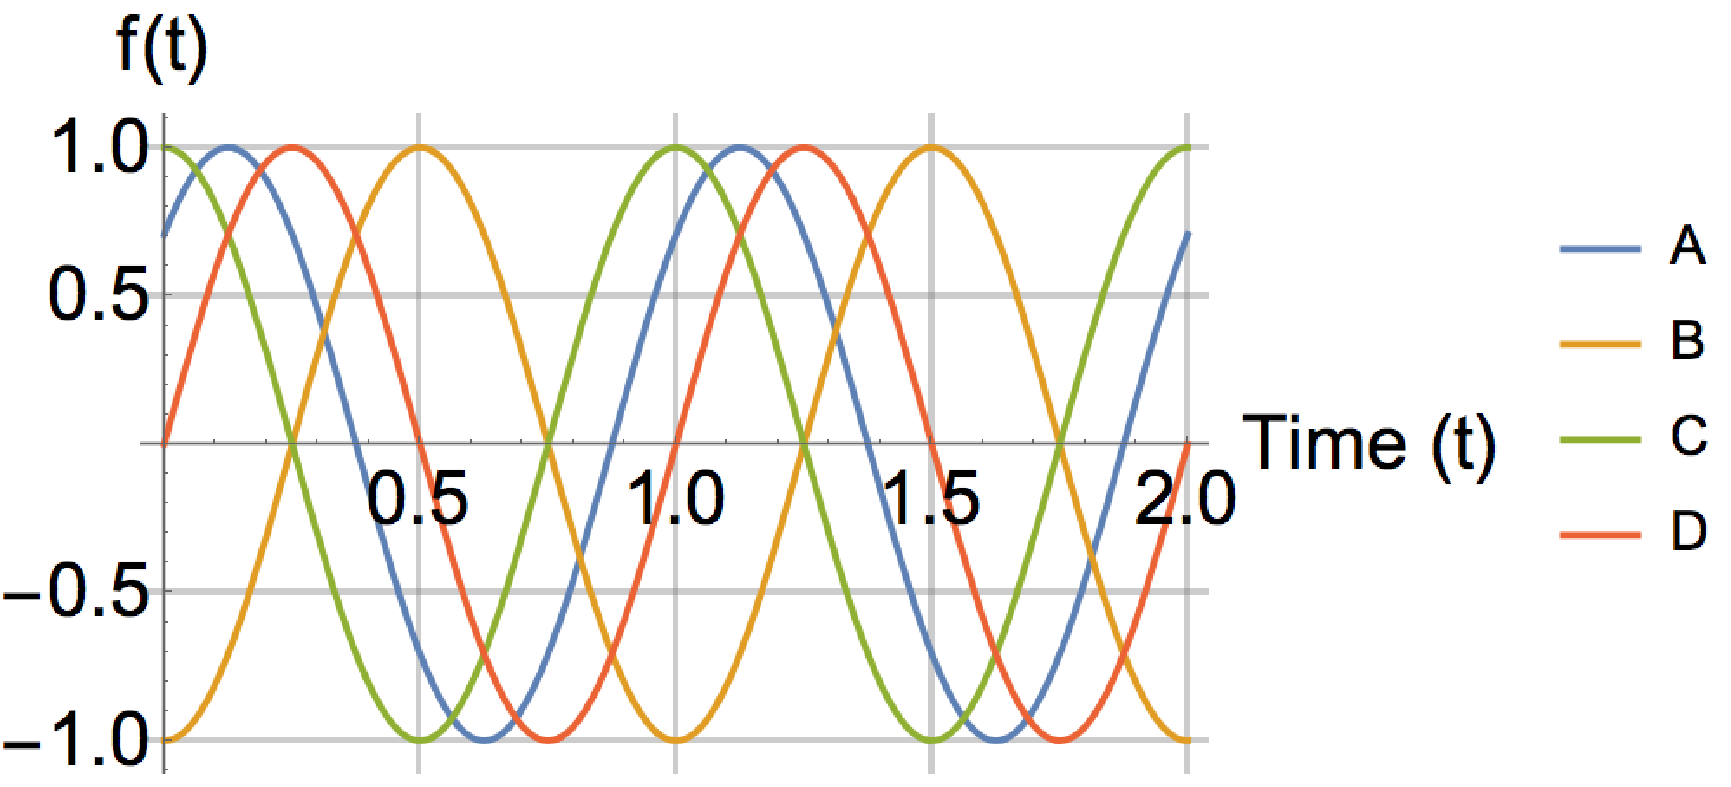
\includegraphics{phase_shift.png}

\subsection*{Solution}
\solstr{i}{5c0e8b}



%%%%%%%%%%%%%%%%%%%%%%%%%%%%%%%%%
\newpage
%%%%%%%%%%%%%%%%%%%%%%%%%%%%%%%%%
\section{Amplitude}

\subsection*{Comments}
Another important concept is amplitude. $\sin(2 \pi t)$ has an amplitude of 1, but this can be easily modified to go between $\pm A$ by multiplication with $A$.

\subsection*{Challenge}
The following 4 graphs correspond to the equation $A \sin(2 \pi k t)$ with variation in the values of $A$ and $k$. What is the sum of the values of $A$ for the following graphs? 

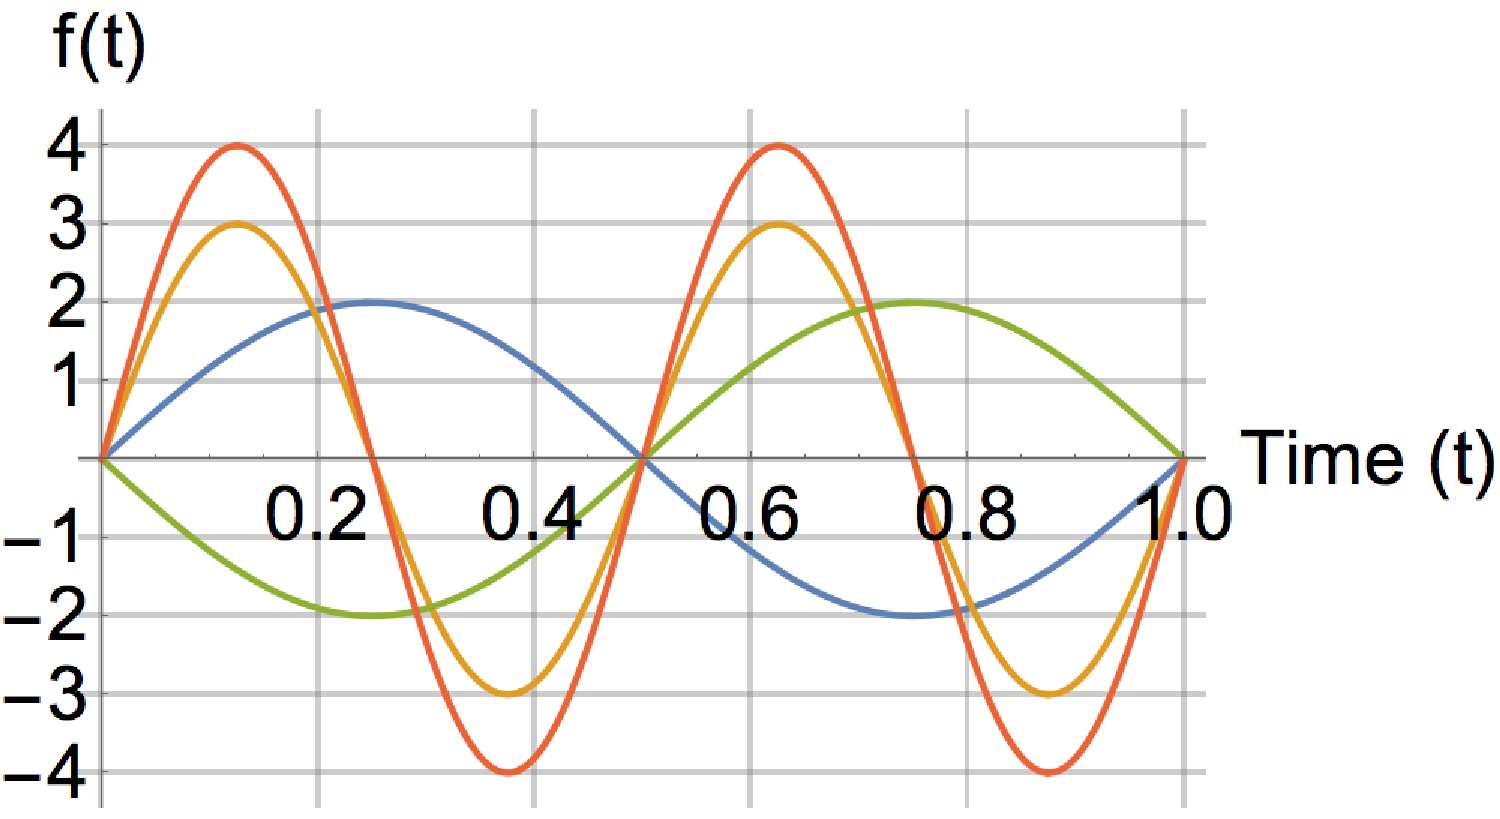
\includegraphics{amplitude.png}

\subsection*{Solution}
\solint{u}{6bce05}




%%%%%%%%%%%%%%%%%%%%%%%%%%%%%%%%%
\newpage
%%%%%%%%%%%%%%%%%%%%%%%%%%%%%%%%%
\section{Periodic and non-periodic signals}
\label{sec:periodic}

\subsection*{Resources}
\begin{itemize}
    \item Video: \url{https://www.youtube.com/watch?v=F_pdpbu8bgA}
    \item Book: 1.3 (\url{https://see.stanford.edu/materials/lsoftaee261/book-fall-07.pdf})
\end{itemize}

\subsection*{Challenge}
The list below contains periodic and non-periodic signals. Sum the points of the signals below that are \emph{periodic}.

1 point: $x(t) = t^2$\\
2 points: $x(t) = \sin(t)$\\
4 points: $x(t) = \sin(2 \pi t)$\\
8 points: $x(t) = \sin(2 \pi t + t)$\\
16 points: $x(t) = \sin(2 \pi t) + \sin(t)$\\
32 points: $x(t) = \sin(5 \pi t) + \sin(2 \pi t)$\\
64 points: $x(t) = \sin(5 \pi t) + \sin(37 \pi t)$\\
128 points: $x(t) = \sin(5 \pi t) + \sin(37.01 \pi t)$\\
256 points: $x(t) = \sin(5 \pi t) + \sin(\sqrt{2} \pi t)$\\
512 points: $x(t) = \sin(5 \sqrt{2} \pi t) + \sin(\sqrt{2} \pi t)$

\subsection*{Solution}
\solint{u}{5d906b}




%%%%%%%%%%%%%%%%%%%%%%%%%%%%%%%%%
\newpage
%%%%%%%%%%%%%%%%%%%%%%%%%%%%%%%%%
\section{Making non-periodic signals from periodic signals}

\subsection*{Challenge}
It is not immediately intuitive that it is possible to make a non-periodic signal by simply adding two periodic signals. Referring to the previous challenge, in no-more than 1 paragraph, explain how this is possible.

\subsection*{Solution}
Please compare your answer with your partner or ask the teacher in class.




%%%%%%%%%%%%%%%%%%%%%%%%%%%%%%%%%
\newpage
%%%%%%%%%%%%%%%%%%%%%%%%%%%%%%%%%
\section{Fundamental frequency}

\subsection*{Challenge}
Considering the periodic signals in challenge \ref{sec:periodic} in order of increasing point-score, calculate the fundamental frequency and period of the last periodic signal in the list.

\subsection*{Solution}
Frequency (Hz) (be careful about rounding up or down to 2 decimal places):\\
\soltwodp{a}{ac6698}

Period (s):\\
\soltwodp{b}{6fdff9}

\chapter{Fourier Series}
\section{Introduction to Fourier coefficients}
\label{sec:fouriercoeffintro}

\subsection*{Resources}
\begin{itemize}
    \item Book: 1.4 (\url{https://see.stanford.edu/materials/lsoftaee261/book-fall-07.pdf})
    \item Video: Lecture 2 (\url{https://www.youtube.com/watch?v=1rqJl7Rs6ps})
\end{itemize}

\subsection*{Challenge}
Deduce in a simple way the Fourier coefficients $a_1$ and $b_1$ in the Fourier series
\begin{equation}
    \sum_{k=1}^{N} a_k cos(2 \pi k t) + b_k sin(2 \pi k t)
\end{equation}

for a signal made up of multiple sine signals
\begin{equation}
    \sum_{k=1}^{N} A_k sin(2 \pi k t + \phi_k)
\end{equation}

for the following cases:
\begin{enumerate}
    \item $N=1$, $k=1$, $A_1=1$, $\phi_1=0$
    \item $N=1$, $k=1$, $A_1=1$, $\phi_1=\pi/2$
    \item $N=1$, $k=1$, $A_1=1$, $\phi_1=\pi/5$
\end{enumerate}

Hint: Using $sin(A+B) = sin(A) cos(B) + cos(A) sin(B)$ it should is possible to find the answer without resorting to complex calculation.

\subsection*{Solutions}
\begin{enumerate}
    \item MD5(o\_$a_k$) = a2c1fe\ldots, MD5(p\_$b_k$) = de80c6\ldots
    \item MD5(a\_$a_k$) = 718a6c\ldots, MD5(s\_$b_k$) = f86f0c\ldots
    \item MD5(d\_$a_k$) = 93d647\ldots, MD5(f\_$b_k$) = 9a7b58\ldots
\end{enumerate}

\timebox




%%%%%%%%%%%%%%%%%%%%%%%%%%%%%%%%%
\newpage
%%%%%%%%%%%%%%%%%%%%%%%%%%%%%%%%%

\section{Even and odd functions}

\subsection*{Resources}
\begin{itemize}
    \item Wikipedia: \url{https://en.wikipedia.org/wiki/Even_and_odd_functions}
\end{itemize}

\subsection*{Challenge}
Referring in part to the cases in challenge \ref{sec:fouriercoeffintro}, sum the points of all the following TRUE statements:

1 point: Case 1 is an odd function

2 points: Case 1 is an even function

4 points: Case 2 is an odd function

8 points: Case 2 is an even function

16 point: Case 3 is an odd function

32 points: Case 3 is an even function

64 points: $f(x)=Sin(x)$ is an odd function

128 points: $f(x)=Sin(x)$ is an even function

256 points: $f(x)=Cos(x)$ is an odd function

512 points: $f(x)=Cos(x)$ is an even function

1024 points: $f(x)=x$ is an odd function

2048 points: $f(x)=x$ is an even function

\subsection*{Solution}
X

\hash{g}{6a18c0}

\timebox




%%%%%%%%%%%%%%%%%%%%%%%%%%%%%%%%%
\newpage
%%%%%%%%%%%%%%%%%%%%%%%%%%%%%%%%%

\section{Fourier Coefficients of sin(x)}
\label{sec:fcsinx}

\subsection*{Resources}
\begin{itemize}
    \item Book: 1.4 (\url{https://see.stanford.edu/materials/lsoftaee261/book-fall-07.pdf})
    \item Video: Lecture 2 (\url{https://www.youtube.com/watch?v=1rqJl7Rs6ps})
\end{itemize}

\subsection*{Comments}
You should be able to follow the derivation of the formula for Fourier coefficients ($C_k$'s) in the video. Feel free to seek help if you have trouble.

\subsection*{Challenge}
By writing $sin(x)$ in exponential form, deduce the Fourier coefficients ($C_k$'s) for the function $sin(x)$, for the following cases:
\begin{enumerate}
    \item k = -1
    \item k = 0
    \item k = 1
\end{enumerate}

\subsection*{Solutions}
\subsubsection{k=-1}
X

\hash{h}{28f251}

\subsubsection{k=0}
X

\hash{j}{4fd3f6}

\subsubsection{k=1}
X

\hash{k}{e82a2a}

\timebox




%%%%%%%%%%%%%%%%%%%%%%%%%%%%%%%%%
\newpage
%%%%%%%%%%%%%%%%%%%%%%%%%%%%%%%%%

\section{Fourier Coefficients of 1 + sin(x)}

\subsection*{Resources}
\begin{itemize}
    \item Book: 1.4 (\url{https://see.stanford.edu/materials/lsoftaee261/book-fall-07.pdf})
    \item Video: Lecture 2 (\url{https://www.youtube.com/watch?v=1rqJl7Rs6ps})
\end{itemize}

\subsection*{Comments}
You should be able to follow the derivation of the formula for Fourier coefficients in the video. Feel free to seek help if you have trouble.

\subsection*{Challenge}
Continuing from challenge \ref{sec:fcsinx}, deduce the Fourier coefficients ($C_k$'s) for the function $1+sin(x)$, for the following cases:
\begin{enumerate}
    \item k = -1
    \item k = 0
    \item k = 1
\end{enumerate}

\subsection*{Solutions}
\subsubsection{k=-1}
X

\hash{z}{39e026}

\subsubsection{k=0}
X

\hash{x}{0ef183}

\subsubsection{k=1}
X

\hash{c}{89b992}

\timebox




%%%%%%%%%%%%%%%%%%%%%%%%%%%%%%%%%
\newpage
%%%%%%%%%%%%%%%%%%%%%%%%%%%%%%%%%

\section{Relation of positive and negative Fourier coefficients for a real signal}

\subsection*{Resources}
\begin{itemize}
    \item Book: 1.4 (\url{https://see.stanford.edu/materials/lsoftaee261/book-fall-07.pdf})
    \item Video: Lecture 2 (\url{https://www.youtube.com/watch?v=1rqJl7Rs6ps})
\end{itemize}

\subsection*{Challenge}
If the Fourier coefficient $C_1$ is $4 + 6i$, what is the Fourier coefficient $C_{-1}$?

\subsection*{Solution}
X

\hash{m}{36ab38}

\timebox




%%%%%%%%%%%%%%%%%%%%%%%%%%%%%%%%%
\newpage
%%%%%%%%%%%%%%%%%%%%%%%%%%%%%%%%%

\section{Converting between trigonometric and exponential forms}
\label{sec:trigexpconvert}

\subsection*{Resources}
\begin{itemize}
    \item Book: 1.4 (\url{https://see.stanford.edu/materials/lsoftaee261/book-fall-07.pdf})
    \item Video: Lecture 2 (\url{https://www.youtube.com/watch?v=1rqJl7Rs6ps})
\end{itemize}

\subsection*{Challenge}
Derive an expression for $C_k$ in terms of the $a_k$'s and $b_k$'s in the expression
\begin{equation}
    f(t) = \frac{a_0}{2} + \sum_{k=1}^{k=N} a_k cos(2 \pi k t) + b_k sin(2 \pi k t) = \sum_{k=-N}^{k=N} C_k e^{2 \pi i k t}
\end{equation}

To check your answer, substitute $a_0 = 1$, $a_1 = 3$ and $b_1 = 5$ as required to calculate $C_k$ for k = -1, 0 and 1.

\subsection*{Solutions}
\subsubsection{k=-1}
X

\hash{v}{052df3}

\subsubsection{k=0}
X

\hash{b}{fb29ff}

\subsubsection{k=1}
X

\hash{n}{284b53}

\timebox




%%%%%%%%%%%%%%%%%%%%%%%%%%%%%%%%%
\newpage
%%%%%%%%%%%%%%%%%%%%%%%%%%%%%%%%%

\section{The Fourier series of $f(t)=t$: $C_0$}

\subsection*{Resources}
\begin{itemize}
    \item Book: 1.5, 1.7 (\url{https://see.stanford.edu/materials/lsoftaee261/book-fall-07.pdf})
    \item Video: Lecture 3 (\url{https://www.youtube.com/watch?v=BjBb5IlrNsQ})
\end{itemize}

\subsection*{Challenge}
Considering the function $f(t)=t$ over the interval 0 to 1, calculate the Fourier coefficient $C_0$ using the derived formula for Fourier coefficients. Compare with the average over the interval.

\subsection*{Solution}
X

\hash{aa}{2708ad}

\timebox




%%%%%%%%%%%%%%%%%%%%%%%%%%%%%%%%%
\newpage
%%%%%%%%%%%%%%%%%%%%%%%%%%%%%%%%%

\section{The Fourier series of $f(t)=t$: $C_k$}

\subsection*{Resources}
\begin{itemize}
    \item Book: 1.5, 1.7 (\url{https://see.stanford.edu/materials/lsoftaee261/book-fall-07.pdf})
    \item Video: Lecture 3 (\url{https://www.youtube.com/watch?v=BjBb5IlrNsQ})
\end{itemize}

\subsection*{Challenge}
Considering the function $f(t)=t$, calculate a general expression for the Fourier coefficients $C_k$ where $k \ne 0$.

To check your answer, evaluate the Fourier coefficient for $k=-30$.

\subsection*{Solution}
X

\hash{bb}{e904e9}

\timebox




%%%%%%%%%%%%%%%%%%%%%%%%%%%%%%%%%
\newpage
%%%%%%%%%%%%%%%%%%%%%%%%%%%%%%%%%

\section{The Fourier series of $f(t)=t$ in exponential form}
\label{sec:fstexpform}

\subsection*{Resources}
\begin{itemize}
    \item Book: 1.4 (\url{https://see.stanford.edu/materials/lsoftaee261/book-fall-07.pdf})
    \item Video: Lecture 3 (\url{https://www.youtube.com/watch?v=BjBb5IlrNsQ})
\end{itemize}

\subsection*{Challenge}
Write the function $f(t)=t$ in terms of its infinite exponential Fourier series.

To check your answer, evaluate the Fourier series up to $n=2$ with $t=0.8$.

The graph with increasing values of $n$ looks like this:

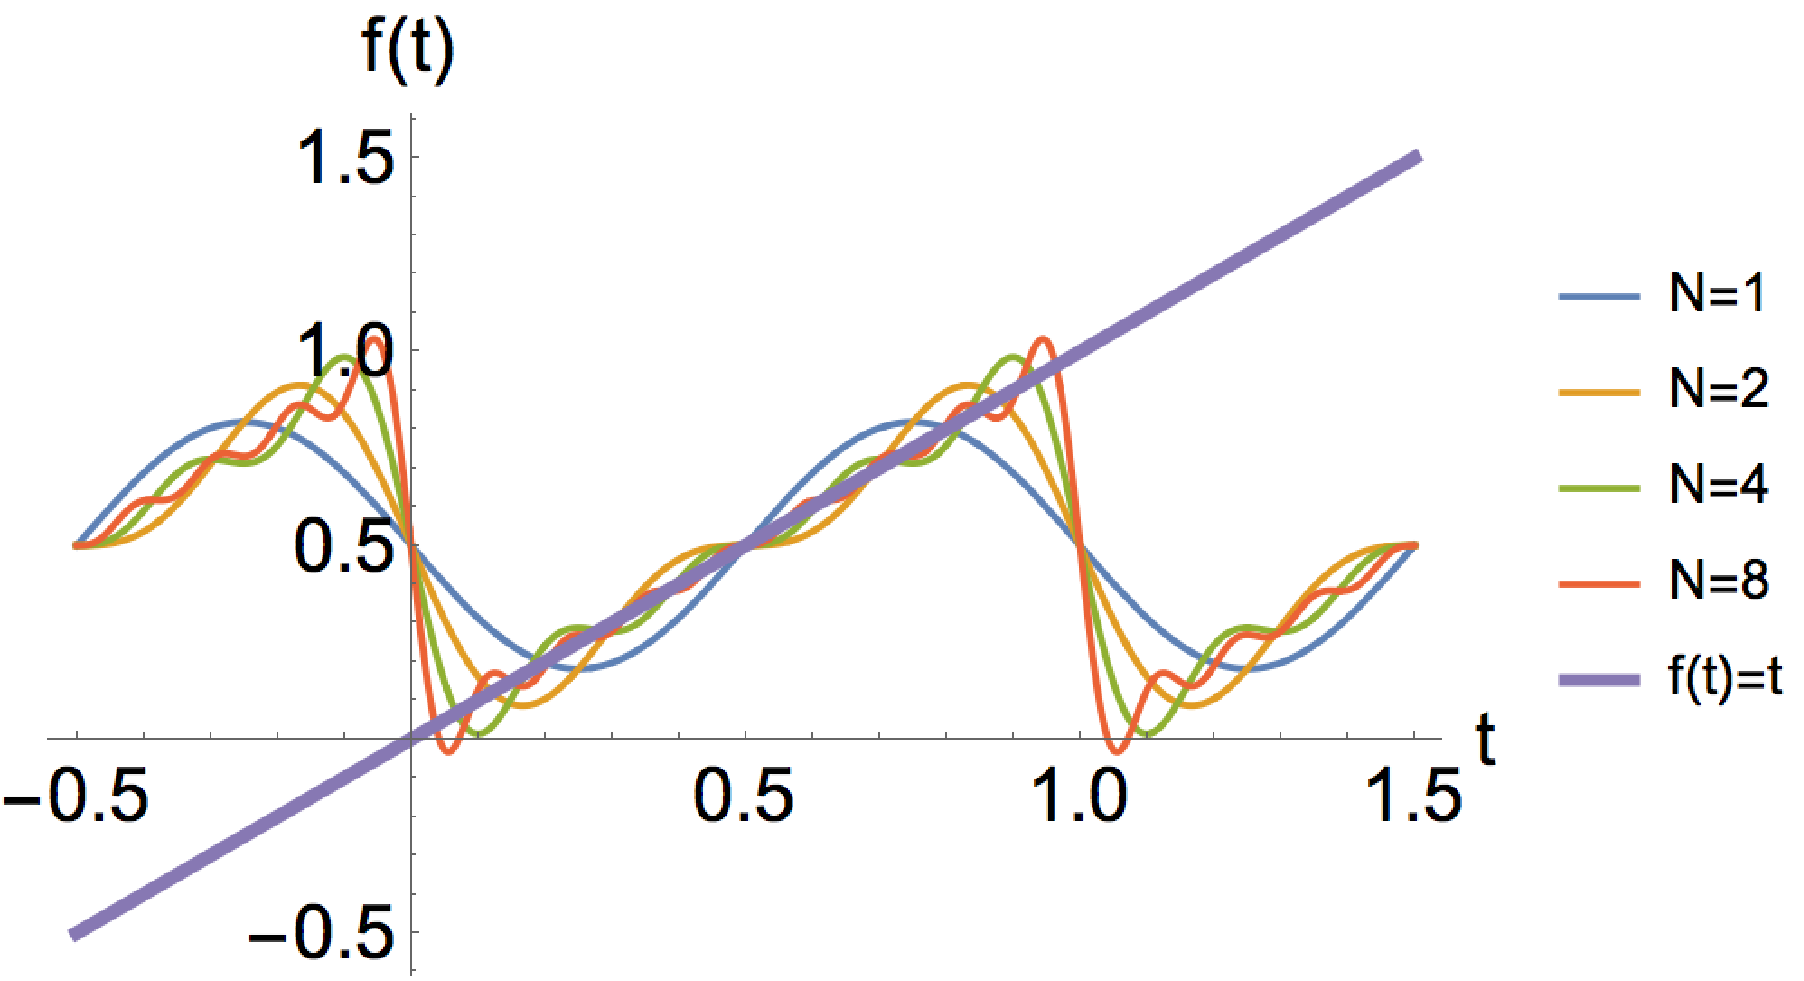
\includegraphics{fourier_series_t.png}

\subsection*{Solution}
X

\hash{cc}{d21e19}

\timebox




%%%%%%%%%%%%%%%%%%%%%%%%%%%%%%%%%
\newpage
%%%%%%%%%%%%%%%%%%%%%%%%%%%%%%%%%

\section{The Fourier series of $f(t)=t$ in trigonometric form}

\subsection*{Resources}
\begin{itemize}
    \item Book: 1.5, 1.7 (\url{https://see.stanford.edu/materials/lsoftaee261/book-fall-07.pdf})
    \item Video: Lecture 2 (\url{https://www.youtube.com/watch?v=1rqJl7Rs6ps})
\end{itemize}

\subsection*{Comment}
Many textbooks will work in terms of ``Fourier sine series'' and ``Fourier cosine series''. For a function that is perfectly even or odd, it is possible to write a Fourier series using one of these two forms. There are direct approaches to calculating sine and cosine Fourier series, in contrast to the route taken here via the exponential form. We will continue to work in the exponential form however, since not only does this provide a deeper understanding, but you can always easily switch between exponential and trigonometric forms if you really want to.


\subsection*{Challenge}
Re-write the series obtained in challenge \ref{sec:fstexpform} in terms of a trigonometric infinite series (ie, using sines and cosines).

To check your answer, evaluate the Fourier series up to $n=2$ with $t=0.8$ and ensure that you get the same answer as you did for challenge \ref{sec:fstexpform}.

\timebox




%%%%%%%%%%%%%%%%%%%%%%%%%%%%%%%%%
\newpage
%%%%%%%%%%%%%%%%%%%%%%%%%%%%%%%%%
\section{Periods other than unity}

\subsection*{Resources}
\begin{itemize}
    \item Book: 1.6 (\url{https://see.stanford.edu/materials/lsoftaee261/book-fall-07.pdf})
\end{itemize}

\subsection*{Challenge}
Determine the Fourier series for the same function as in \ref{sec:fstexpform} ($f(t)=t$), except approximate the function over the region $1<x<3$ instead of $0<x<1$.

To check your answer, evaluate the Fourier series up to $n=2$ with $t=1.8$.

The graph with increasing values of $n$ looks like this:

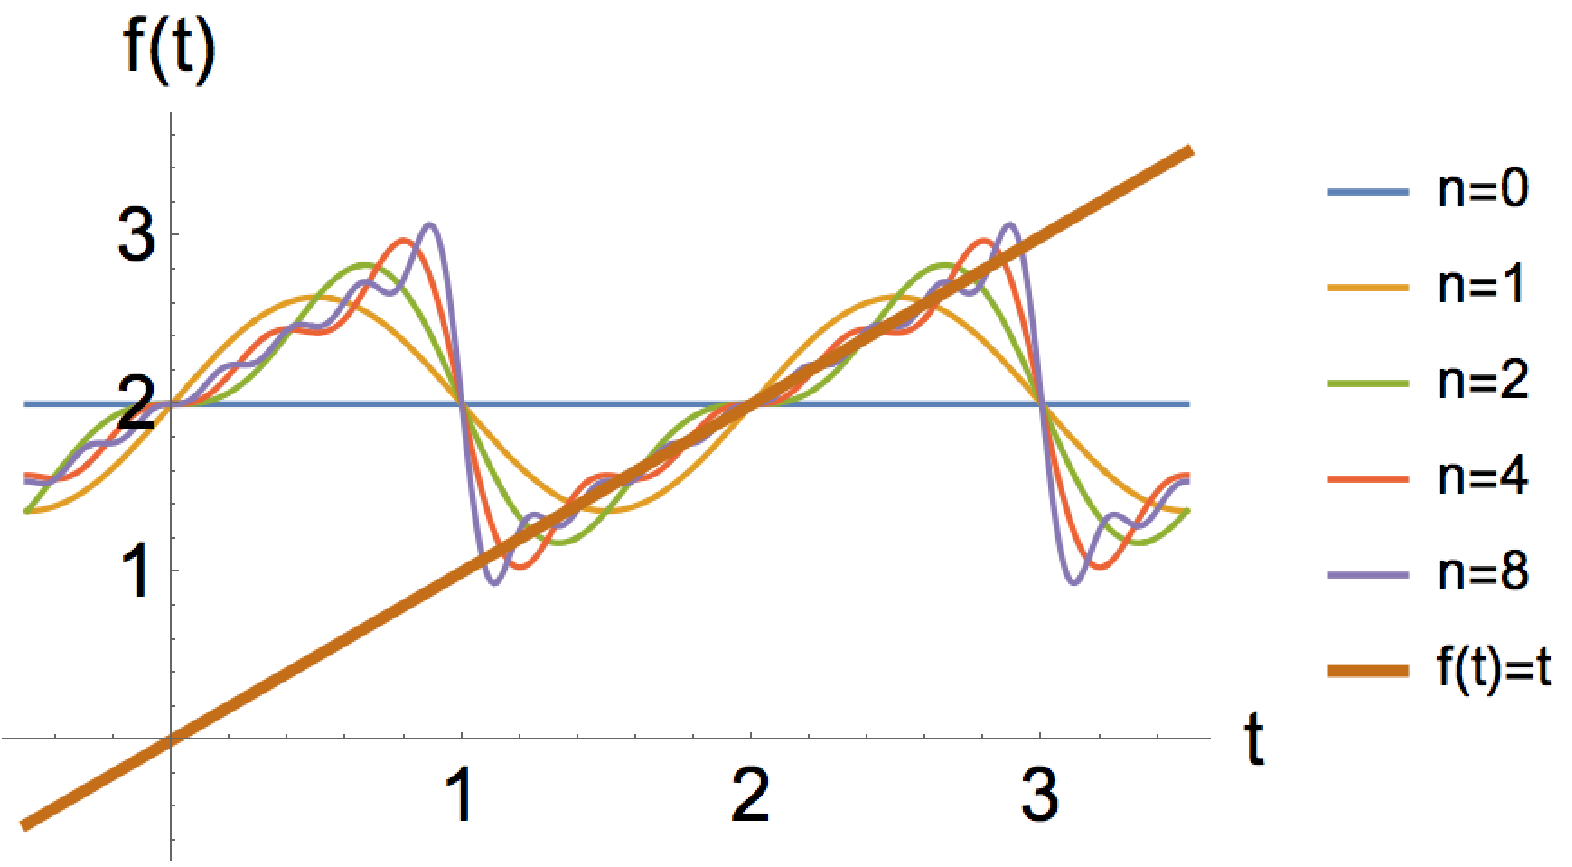
\includegraphics{fs_other_periods.png}

\subsection*{Solution}
X

\hash{dd}{83e943}

\timebox




%%%%%%%%%%%%%%%%%%%%%%%%%%%%%%%%%
\newpage
%%%%%%%%%%%%%%%%%%%%%%%%%%%%%%%%%
\section{Infinite series}

\subsection*{Comment}
It is important to understand why some series are infinite, while others are not (well, technically all series are infinite since they all involve sums to $n=\infty$, however for some series the Fourier coefficients are all zero above a certain value of $n$). Therefore, make sure you understand why the answer is as it is, below. If you don't, be sure to discuss with others.

\subsection*{Challenge}
The Fourier series is a sum to $\pm \infty$, however in some cases the coefficients ($C_k$'s) are zero beyond a certain number of terms. Which of the terms below will have Fourier coefficients that are all zero after a certain number of terms? Sum the points of these functions.

1 point: $x$

2 points: $x^2$

4 points: $cos(2 x) + 3 sin(7 x)$

8 points: $e^{2 \pi i x}$

\subsection*{Solution}
X

\hash{ee}{8e05a4}

\timebox




%%%%%%%%%%%%%%%%%%%%%%%%%%%%%%%%%
\newpage
%%%%%%%%%%%%%%%%%%%%%%%%%%%%%%%%%
\section{k-symmetry}

\subsection*{Challenge}
Determine what X and Y represent algebraically.
\begin{equation}
    cos(k \pi t) = \frac{1}{2} e^{-k i\pi t} + \frac{1}{2} e^{\bm{X} i \pi x}
\end{equation}
\begin{equation}
    sin(k \pi t) = \frac{1}{2} i e^{\bm{Y} i \pi t} - \frac{1}{2} i e^{k i \pi t}
\end{equation}

To check your answers you may substitute any appropriate values from the following list: $k=2$, $t=1$

\subsection*{Solution}
X

\hash{ff}{942d6f}

Y

MD5(gg\_Y) = a379b8\ldots

\timebox




%%%%%%%%%%%%%%%%%%%%%%%%%%%%%%%%%
\newpage
%%%%%%%%%%%%%%%%%%%%%%%%%%%%%%%%%
\section{Direct trigonometric calculation of a Fourier series: the coefficients}
\label{sec:fs_squarewave}

\section*{Comment}
This challenge introduces several key concepts at once, including decoupling of integral intervals and periodicity, the concept of a square wave and direct trigonometric evaluation of Fourier series. If you can master this you'll be in a really strong position.

It is hopefully clear now that for real signals, due to the symmetry of the positive and negative k's, one can fully compose Fourier series in terms of sine and cosine. In challenge \ref{sec:trigexpconvert} we saw the formula for the function in terms of Fourier coefficients $a_0$, $a_n$ and $b_n$. While we will not use this approach, it is important to be able to utilise such a formulation since this is the way some books present it and some people have learnt it. Therefore, without proof, the coefficients can be calculated using

\begin{equation}
    a_k = \frac{2}{T} \int_{t_0}^{t_0+T} f(t) Cos(2 \pi k t/T)
\end{equation}
\begin{equation}
    b_k = \frac{2}{T} \int_{t_0}^{t_0+T} f(t) Sin(2 \pi k t/T)
\end{equation}

\subsection*{Challenge}
Using the direct trigonometric Fourier series, obtain a general expression for the $a_k$ and $b_k$ coefficients for the square-wave signal with periodicity 4

\begin{equation}
    f(t)=
    \begin{cases}
        1 & \text{for } -1<t<1 \\
        0 & \text{for } 1<t<3
    \end{cases}
\end{equation}

A graph of the function, including the solution for various values of $n$, is shown here:

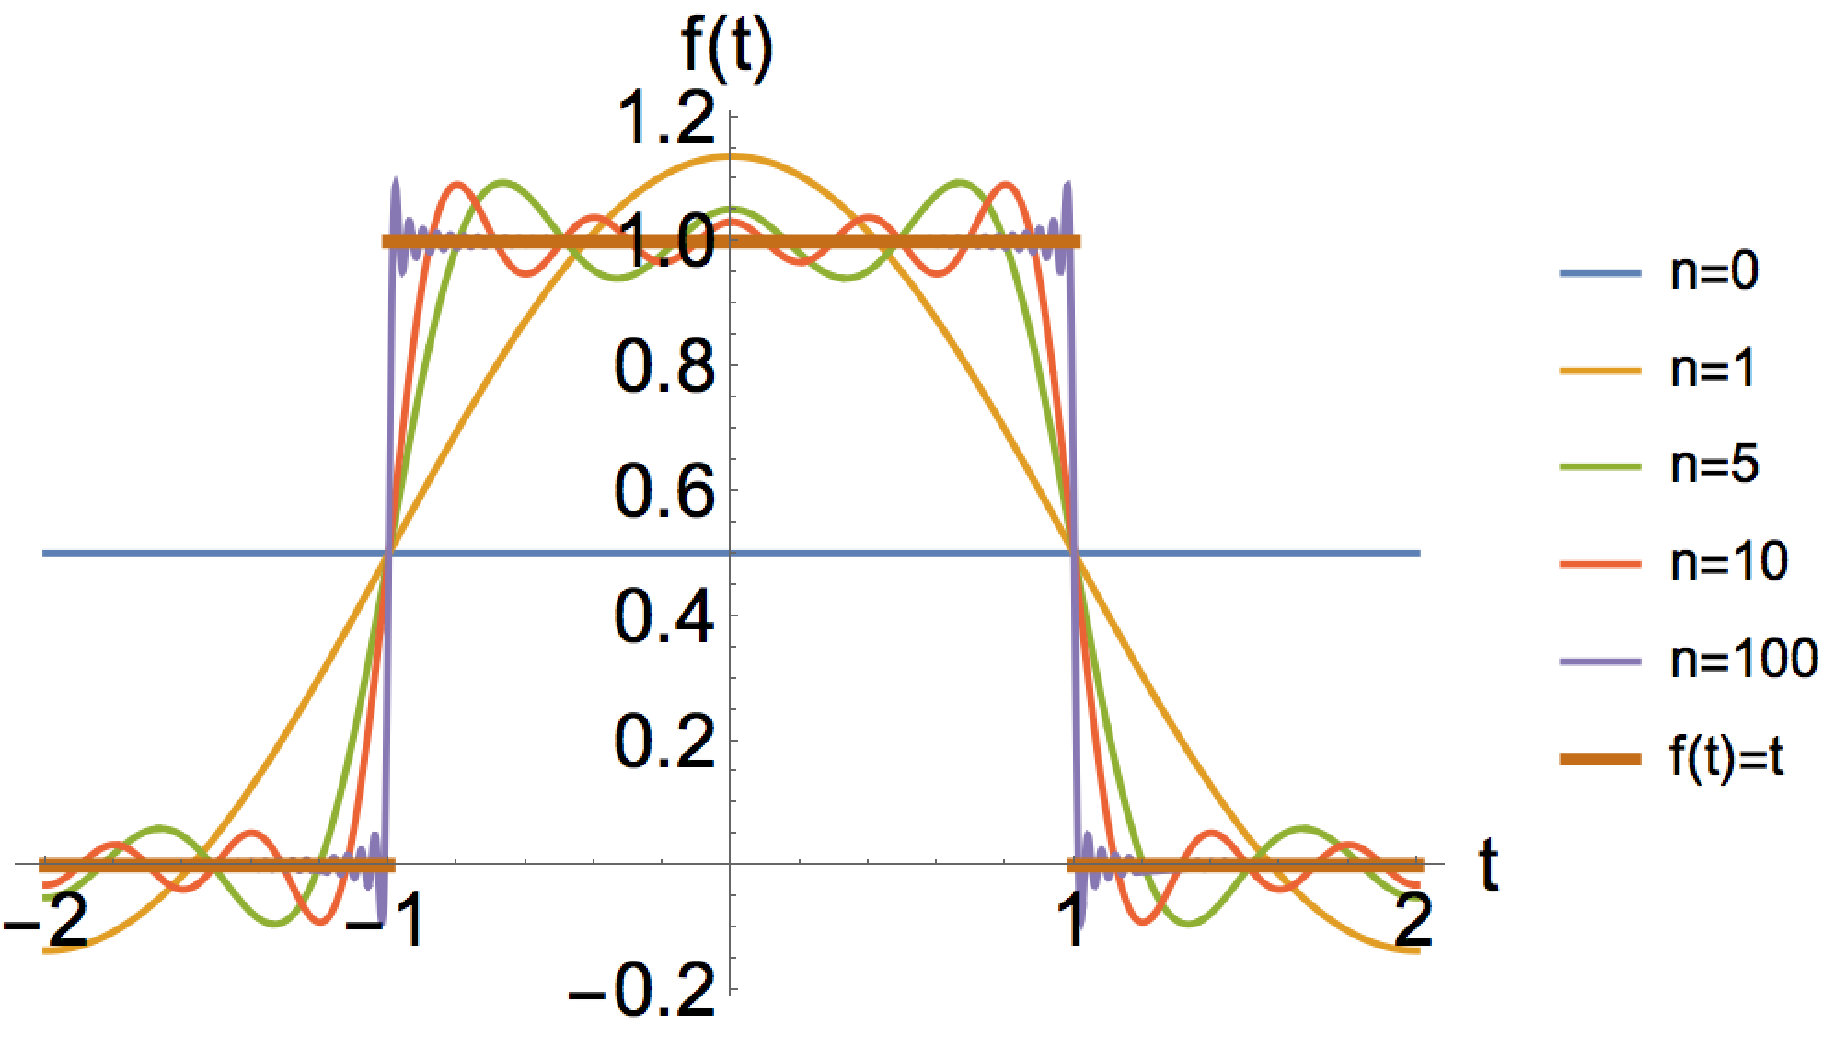
\includegraphics{fs_square_wave.png}

Note the symmetry of the problem. Can you see what terms will be zero? To check your solution, calculate $a_k$ and $b_k$ for $k=0$, $k=2$ and $k=3$. Also note that you will have to break the integrals into two parts and sum them in order to tackle this problem.

\subsection*{Solution}
\begin{tabular}{|l|l|l|}
    \hline
    $k$ & $a_k$ & $b_k$ \\
    \hline
    0 & MD5(hh\_X)=e57c15\ldots & MD5(ii\_X)=377fe2\ldots \\
    2 & MD5(jj\_X)=54aaa1\ldots & MD5(kk\_X)=be063f\ldots \\
    3 & MD5(mm\_X)=b8fce7\ldots & MD5(nn\_X)=b6fbaf\ldots \\
    \hline
\end{tabular}

\timebox




%%%%%%%%%%%%%%%%%%%%%%%%%%%%%%%%%
\newpage
%%%%%%%%%%%%%%%%%%%%%%%%%%%%%%%%%
\section{Direct trigonometric calculation of a Fourier series: the series}

\subsection*{Challenge}
Calculate the Fourier series for the square wave introduced in challenge \ref{sec:fs_squarewave} using direct trigonometric calculation for up to $n=3$. Check your solution by evaluating for $t=0.1$.

\subsection*{Solution}
\six{}

\hash{oo}{bd7e5e}

\timebox




%%%%%%%%%%%%%%%%%%%%%%%%%%%%%%%%%
\newpage
%%%%%%%%%%%%%%%%%%%%%%%%%%%%%%%%%
\section{2D orthogonal vectors}

\subsection*{Resources}
\begin{itemize}
    \item Book: 1.9 (\url{https://see.stanford.edu/materials/lsoftaee261/book-fall-07.pdf})
\end{itemize}

\subsection*{Challenge}
Sum the points of the vectors in 2D that are orthogonal:

1 point: (5, 4) and (-1, 1.25)

2 points:  (2, -3) and (-6, 4)

4 points: (-2.25, 1.5) and (2, 3)

8 points: (4.5, 4) and (3, -3.375)

16 points: (6, 4) and (4, -6)

32 points: (5, 1) and (-2, 8.125)

64 points: (0, 1) and (1, 0)

128 points: (1, 1) and (1, 1)

\subsection*{Solution}
\six{}

\hash{pp}{92843f}

\timebox




%%%%%%%%%%%%%%%%%%%%%%%%%%%%%%%%%
\newpage
%%%%%%%%%%%%%%%%%%%%%%%%%%%%%%%%%
\section{Orthonormal basis}

\subsection*{Resources}
\begin{itemize}
    \item Video: \url{https://www.khanacademy.org/math/linear-algebra/alternate-bases/orthonormal-basis/v/linear-algebra-introduction-to-orthonormal-bases}
\end{itemize}

\subsection*{Challenge}
Sum the points of the following vectors that form an orthonormal basis:

1 point :
($\displaystyle \frac{1}{\sqrt{5}}, \frac{2}{\sqrt{5}}$) and
($\displaystyle \frac{2}{\sqrt{5}}, \frac{4}{\sqrt{5}}$)

2 points:
($\displaystyle \frac{2}{\sqrt{5}}$, $\displaystyle \frac{1}{\sqrt{5}}$) and
($\displaystyle \frac{-1}{\sqrt{5}}$, $\displaystyle \frac{2}{\sqrt{5}}$)

4 points:
($\displaystyle \frac{2}{\sqrt{2}}, \sqrt{\frac{7}{8}}, \frac{1}{\sqrt{6}}$),
($\displaystyle -\sqrt{\frac{2}{5}}, \frac{7}{\sqrt{14}}, -\frac{1}{\sqrt{6}}$) and
($\displaystyle \frac{1}{\sqrt{3}},  \frac{1}{5 \sqrt{3}}, -\frac{7}{5 \sqrt{3}}$)

8 points:
($\displaystyle \frac{1}{\sqrt{21}}, \frac{2}{\sqrt{21}}, \frac{4}{\sqrt{21}}$),
($\displaystyle -\sqrt{\frac{2}{7}}, \frac{3}{\sqrt{14}}, -\frac{1}{\sqrt{14}}$) and
($\displaystyle \sqrt{\frac{2}{3}},  \frac{1}{\sqrt{6}}, -\frac{1}{\sqrt{6}}$)

16 points:
($\displaystyle \frac{1}{\sqrt{6}}, \sqrt{\frac{2}{3}}, \frac{1}{\sqrt{6}}$),
($\displaystyle -\frac{1}{\sqrt{2}},  \frac{2 \sqrt{2}}{5}, -\frac{3}{5 \sqrt{2}}$) and
($\displaystyle \frac{1}{\sqrt{3}},  \frac{1}{5 \sqrt{3}}, -\frac{7}{5 \sqrt{3}}$)

32 points:
($0, 2$) and ($2, 0$)

64 points:
($0, 1$) and ($1, 0$)

\subsection*{Solution}
\six{}

\hash{qq}{097fd7}

\timebox




%%%%%%%%%%%%%%%%%%%%%%%%%%%%%%%%%
\newpage
%%%%%%%%%%%%%%%%%%%%%%%%%%%%%%%%%
\section{Natural basis}

\subsection*{Resources}
\begin{itemize}
    \item Book: 1.9 (\url{https://see.stanford.edu/materials/lsoftaee261/book-fall-07.pdf})
\end{itemize}

\subsection*{Challenge}
Sum the components of the following vectors of an orthonormal basis in $\mathbb{R}^{300}$ space:

\begin{itemize}
    \item First component of the first vector
    \item first component of the second vector
    \item 200th component of the 100th vector
    \item 200th component of the 200th vector
    \item last component of the 299th vector
    \item last component of the last vector
\end{itemize}

\subsection*{Solution}
\six{}

\hash{rr}{095c77}

\timebox




%%%%%%%%%%%%%%%%%%%%%%%%%%%%%%%%%
\newpage
%%%%%%%%%%%%%%%%%%%%%%%%%%%%%%%%%
\section{Orthonormal basis for Fourier series}

\subsection*{Resources}
\begin{itemize}
    \item Book: 1.9 (\url{https://see.stanford.edu/materials/lsoftaee261/book-fall-07.pdf})
\end{itemize}

\subsection*{Comment}
The previous challenges have focussed on the orthogonality and orthonormality of vectors. We now make the jump to functions. As chapter 1.9 explains, although its not perfect, the analogy between vectors and functions is a good way to help understand and visualise the role that the terms of a Fourier series play in defining a basis upon which to describe a function.

\subsection*{Challenge}
Starting from the inner product of two terms ($e^{2 \pi i k_1 t}$, $e^{2 \pi i k_2 t}$) of a Fourier series, demonstrate that the terms of a Fourier series form an orthonormal basis. \textbf{Show a full derivation}.

To check your intuition, you may evaluate the following cases:

$X = (e^{2 \pi i k_1 t}, e^{2 \pi i k_1 t})$

$Y = (e^{2 \pi i k_1 t}, e^{2 \pi i k_2 t})$

\subsection*{Solution}
If you are not confident about your derivation, please check with someone else. If there is any step that you do not fully understand, do not hesitate to ask. If you do not understand the connection between previous challenges on vectors and this challenge using functions, do not hesitate to ask someone.

\textbf{X}

\hash{ss}{8f7f41}

\textbf{Y}

MD5(tt\_Y) = 2c669b\ldots

\timebox




%%%%%%%%%%%%%%%%%%%%%%%%%%%%%%%%%
\newpage
%%%%%%%%%%%%%%%%%%%%%%%%%%%%%%%%%
\section{Circles and Fourier series}

\subsection*{Resources}
\begin{itemize}
    \item Video 1: \url{https://www.youtube.com/watch?v=Y9pYHDSxc7g}
    \item Video 2: \url{https://www.youtube.com/watch?v=LznjC4Lo7lE}
\end{itemize}

\subsection*{Comment}
In the first lecture we saw how it was possible to approximate any function given enough circles. Here we link what you have learned back to that first lecture. I strongly recommend viewing the fun and informative videos listed here under Resources. In summary, by building a Fourier series you are representing a function using an orthonormal basis, where each component of the basis can be considered visually as a circle operating with individual radius and frequency on the real-imaginary plane. If, after completing this challenge, that last sentence makes sense to you, then you have achieved the first major goal of this course.

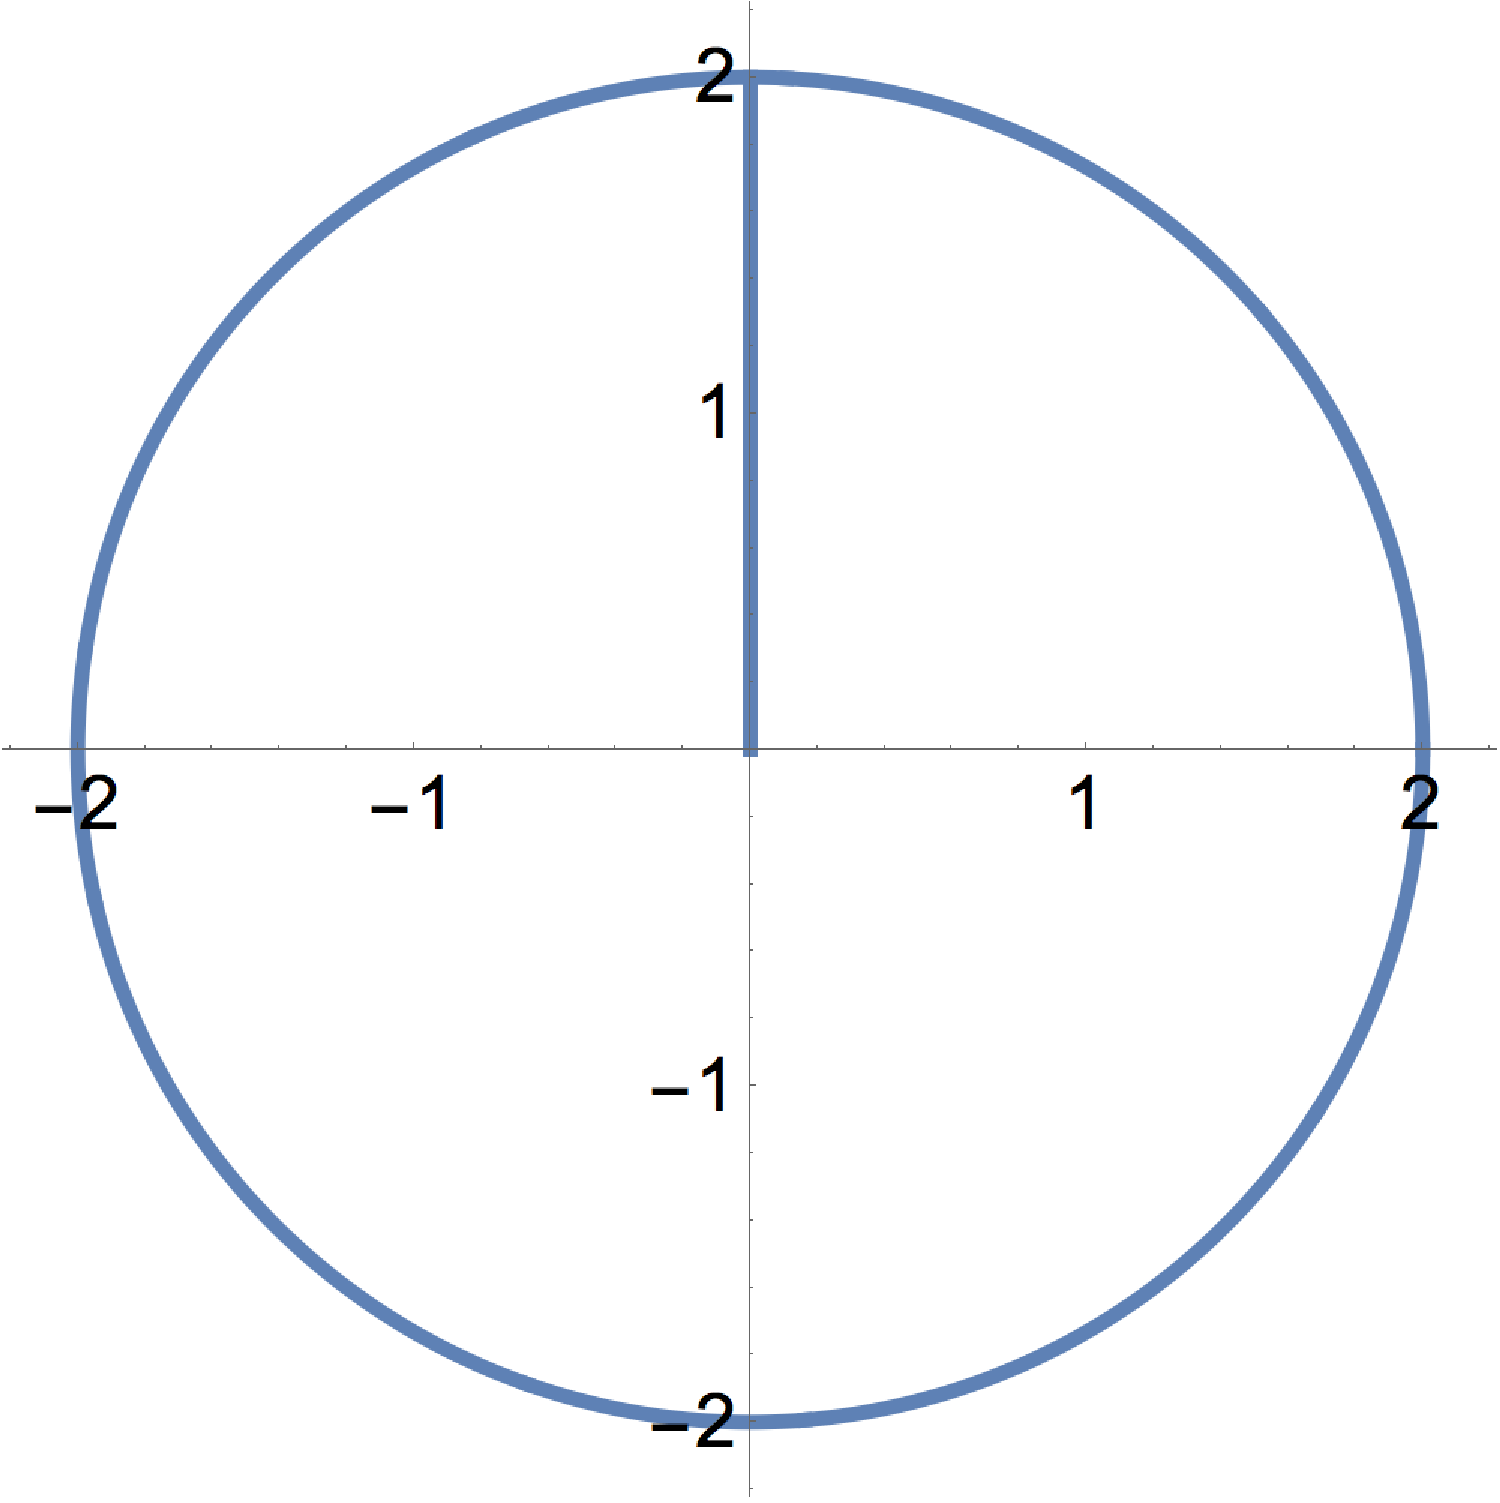
\includegraphics[scale=0.5]{circle.png}

\subsection*{Challenge}
Treating the x-axis as the real axis and the y-axis as the imaginary axis, arrange the equations below in the following order:

\begin{enumerate}
    \item A point moving round on a circle with radius 2 units and frequency 2 Hz
    \item A point moving round on a circle with radius 3 units and frequency 1 Hz
    \item A point moving round on a circle with radius 2 units and a period of 1 second
    \item A point moving round on a circle with radius 3 units and a period of 2 seconds
\end{enumerate}

Equations:

$\displaystyle A e^{2 \pi i k t}$ where $t$ is time in seconds and the values of $A$ and $k$ are as follows:

A: $A=2$, $k=2$ 

B: $A=3$, $k=1$

C: $A=3$, $k=0.5$

D: $A=2$, $k=1$

\subsection*{Solution}
\six{}

\hash{uu}{cb7845}

\timebox

% Convergence?
% Gibbs phenomena?



% Sine and cosine series? Even odd functions?
%\chapter{Fourier Transform (continuous)}
%\chapter{Fourier Transform (discrete)}
% Discrete FT
% FFT
% Zero-padding

% Convolution?
\end{document}
